\documentclass[12pt,a4paper]{article}
\usepackage{bold-extra}
\usepackage{appendix}
\usepackage{amsfonts,amsmath,amssymb}
\usepackage{enumerate}
\usepackage{float}
\usepackage{geometry}
\usepackage{graphicx}
\usepackage{latexsym}
\usepackage{listings}
\usepackage{multicol,multirow}
\usepackage{subfigure}
\usepackage{tabularx}
\usepackage{ulem}
\usepackage{wrapfig}
\usepackage{tikz}
\usepackage{xcolor}
\geometry{a4paper,left=1in,right=1in,top=1in,bottom=1in}
\begin{document}
\centerline{\Huge{{\textbf{PHYSICS I\ \ Problem Set 10}}}}
\vspace{0.5cm}
\leftline{\large{Name: Haotian Fu}}
\rightline{\large{Student ID: 520021910012}}
\section*{\large \textbf{Problem 1}}
{\textbf{Solution}}

Suppose the mass of the ball is $m$ with radius $r$ and the mass of the ring is $M$ with radius $R$.

For the ball
\begin{align}
	\left\{
	\begin{array}{l}		
			ma_{\rm cm,1} = mg\sin\alpha - f_{s,1}\\
			f_{s,1} r = I_1\varepsilon = \frac{2}{5}mr^2\varepsilon\\
			a_{\rm cm,1} = \varepsilon_1 r
	\end{array}
	\right.
\end{align}

For the ring
\begin{align}
	\left\{
	\begin{array}{l}
			Ma_{\rm cm,2} = Mg\sin\alpha - f_{s,2}\\
			f_{s,2} R = I_2\varepsilon = MR^2\varepsilon\\
			a_{\rm cm,2} = \varepsilon_2 R
	\end{array}
	\right.
\end{align}

Then we get
\begin{align}
	\left\{
	\begin{array}{l}
		a_{\rm cm,1} = \frac{5}{7}g\sin\alpha\\
		a_{\rm cm,2} = \frac{1}{2}g\sin\alpha
	\end{array}
	\right.
\end{align}

Since the distance the ball and the ring travel during $t$ period is the same
\begin{align}
	\frac{1}{2}a_{\rm cm,1} t^2 = v_0 t + \frac{1}{2}a_{\rm cm,2} t^2
\end{align}
where $a_{\rm cm,1}$ and $a_{\rm cm,2}$ satisfy Equations(3).

Therefore, we get
\begin{align}
	v_0 = \frac{3}{28}gt\sin\alpha
\end{align}
which is directing downward along the inclined plane

\section*{\large \textbf{Problem 2}}
{\textbf{Solution}}

\begin{enumerate}[(a)]

\item According to FBD in Fig. 1, we have
\begin{align}
	\left\{
		\begin{array}{l}
			T_1 = m_1 a\\
			m_2g - T_2 = m_2 a\\
			T_1 + f_s = T_2\\
			f_s R = I\varepsilon = \frac{1}{2}MR^2\varepsilon\\
			a = R\varepsilon
		\end{array}
	\right.
\end{align}

Soving Equations(6)
\begin{align}
	\left\{
	\begin{array}{l}
		a = \frac{2m_2}{2m_1+2m_2+M}\cdot g\\
		T_1 = \frac{2m_1}{2m_1+2m_2+M}\cdot m_2g\\
		T_2 = \frac{2m_1+M}{2m_1+2m_2+M}\cdot m_2g
	\end{array}
	\right.
\end{align}

\item The acceleration of the box has already been shown in Equations(7). Namely,
$$
	a = \frac{2m_2}{2m_1+2m_2+M}\cdot g \qquad {\rm directing\ to\ the\ right\ or\ downwards}
$$

\item For the pulley, according to FBD, the horizontal force exerted on it is $T_1$ and the vertical force exerted on it is $T_2 + Mg$. Namely,
\begin{align}
	F_{\rm horizontal} &= \frac{2m_1}{2m_1+2m_2+M}\cdot m_2g \qquad {\rm directing\ to\ the\ right}\\
	F_{\rm vertical} &= \frac{2m_1+M}{2m_1+2m_2+M}\cdot m_2g + Mg \qquad {\rm upwards}
\end{align}

\end{enumerate}

\begin{figure}[!htbp] 
\centering 
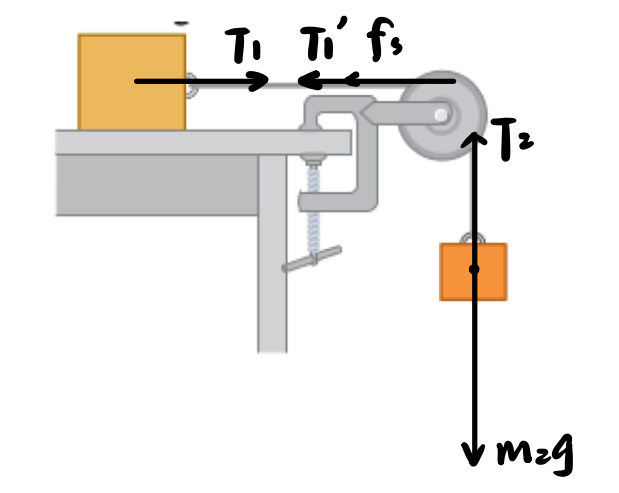
\includegraphics[width=0.4\linewidth]{FDR1.png}  
\caption{Free Body Diagram in Problem 2} 
\end{figure}


\section*{\large \textbf{Problem 3}}
{\textbf{Solution}}

\begin{wrapfigure}{1}[0cm]{0pt}
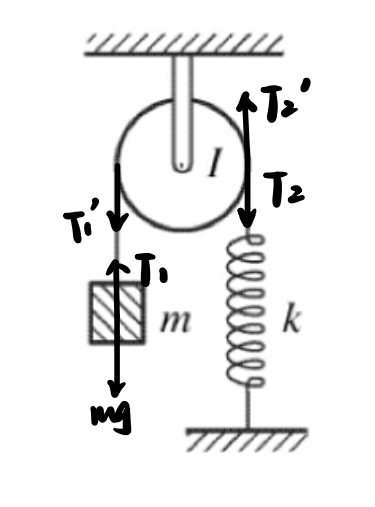
\includegraphics[width=4cm]{FDR2.png}
\caption{Free Body Diagram in Problem 3}
\end{wrapfigure}

According to FBD in Fig. 2, we have
\begin{align}
	\left\{
		\begin{array}{l}
			(T_1-T_2) R = I\varepsilon\\
			mg-T_1 = ma\\
			T_2 = kx\\
			\varepsilon = a/R
		\end{array}
	\right.
\end{align}

Therefore
\begin{align}
	a = \frac{mg-kx}{m+I/R^2}
\end{align}

Since $F=ma \propto x$, the ocsillation is \textbf{SHM}.

Therefore, period of this oscillation is
\begin{align}
	T = 2\pi\sqrt{\frac{mR^2 + I}{kR^2}}
\end{align}



\section*{\large \textbf{Problem 4}}
{\textbf{Solution}}

Definition of impulse
\begin{align}
	J = mv_{\rm cm}
\end{align}

Definition of angular velocity
\begin{align}
	\omega = \frac{v_{\rm cm}}{d}
\end{align}

Second law of dynamics for a rigid body rotating about a fixed axis. For the axis through the end of the bat
\begin{align}
	xF = I\varepsilon
\end{align}

Parallel theorem
\begin{align}
I = I_{\rm cm} + md^2
\end{align}

Ingegrate Equation(15) by $dt$ from $t_1$ to $t_2$
\begin{align*}
	x\int_{t_1}^{t_2} F dt &= I \int_{t_1}^{t_2} \varepsilon dt\\
\Rightarrow \qquad xJ = I\omega &= I\frac{v_{\rm cm}}{d} = \frac{J}{md}
\end{align*}

Therefore, we get
\begin{align}
	x = 0.71\ m
\end{align}


\end{document}